\section{PID-Regler}

\begin{outline}
    \1 \textbf{P}: Proportional $K_P \cdot e(t)$
        \2 Gegenwart: Gewichtung des \textbf{aktuellen} Fehlers $e(t)$
            \3 Stellgrösse $u(t)$ ist abhängig vom aktuell vorhandenen Fehler
            \3 Wie gross Fehler in Vergangenheit war oder in welche Richtung er sich entwickelt, ist irrelevant
    \1 \textbf{I}: Integral $K_I \int e(t)$
        \2 Vergangenheit: Gewichtung der \textbf{Summe vergangener} Fehler
            \3  Stellgrösse $u(t)$ ist abhängig davon, wie lange ein Fehler schon existiert
            \3 Wie gross der aktuelle Fehler ist und wie start er sich gerade ändert, ist irrelevant
    \1 \textbf{D}: Differential $K_D \cdot \dot{e}(t)$
        \2 Zukunft, Trend: Gewichtung der \textbf{Änderung} des Fehlers
            \3 Stellgrösse ist abhängig davon, wie stark der Fehler gerade zu-/abnimmt
            \3 Wie gros der aktuelle Fehler ist und wie lange er schon existiert, ist irrelevant
\end{outline}


\subsection{Strukturen und Frequenzgänge von PID-Reglern}
\label{Strukturen PID-Regler}

Alle drei Strukturen sind \textbf{äquivalent}. Es handelt sich nur um unterschiedliche Darstellungsformen.


\subsubsection{Varirante 1: Parallelform}

\begin{minipage}[c]{0.4\columnwidth}
    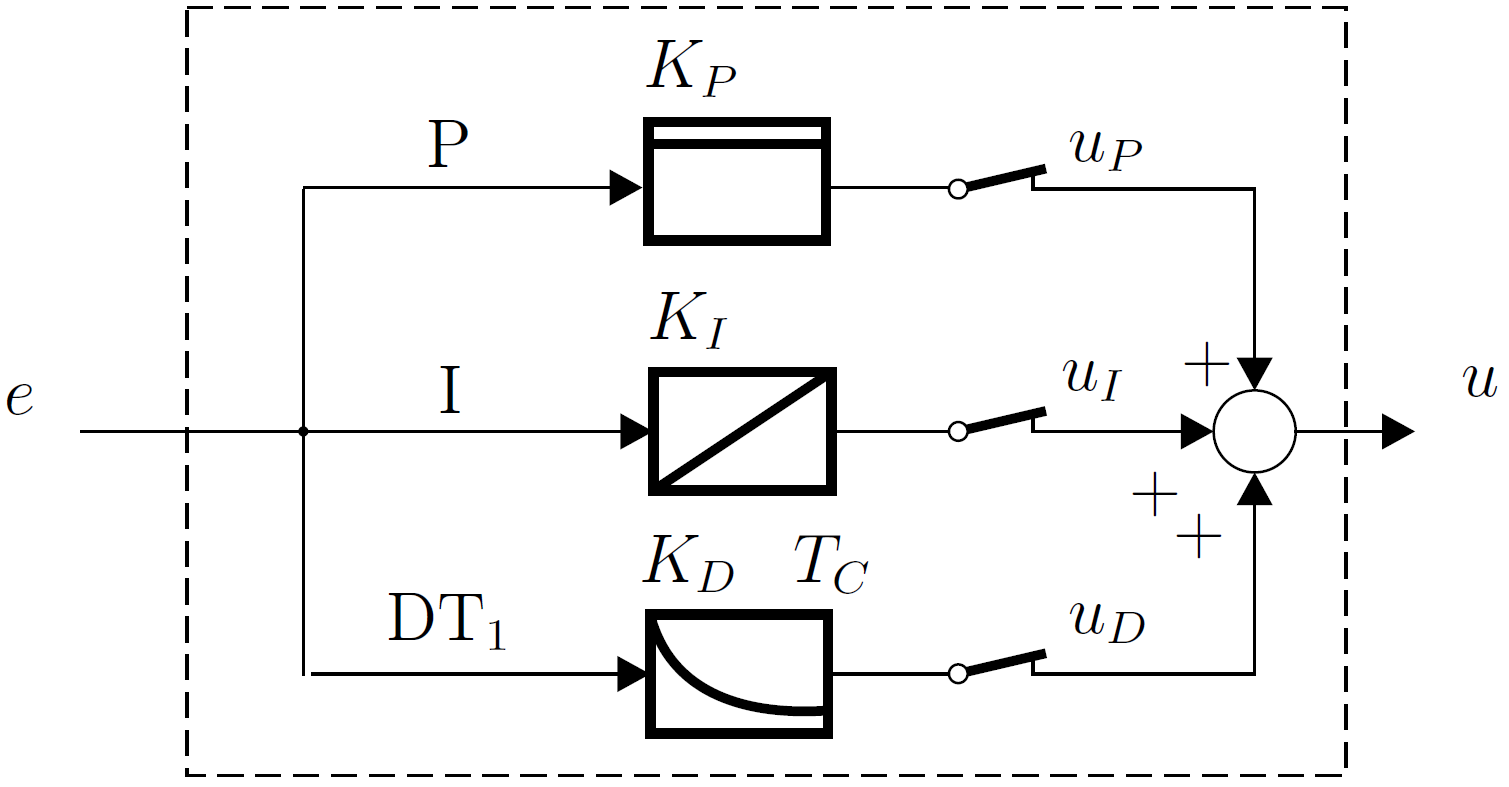
\includegraphics[width=\columnwidth]{images/pid_regler_aufbau.png}
\end{minipage}
\hfill
\begin{minipage}[c]{0.48\columnwidth}
    $$ \boxed{ G_{\rm PID}(\jimg \omega) = K_P + \frac{K_I}{\jimg \omega} + K_D \frac{\jimg \omega}{1 + \jimg \omega T_C} } $$
\end{minipage}


\subsubsection{Variante 2: Standardform (P-Anteil vorangestellt)}

\begin{minipage}[c]{0.4\columnwidth}
    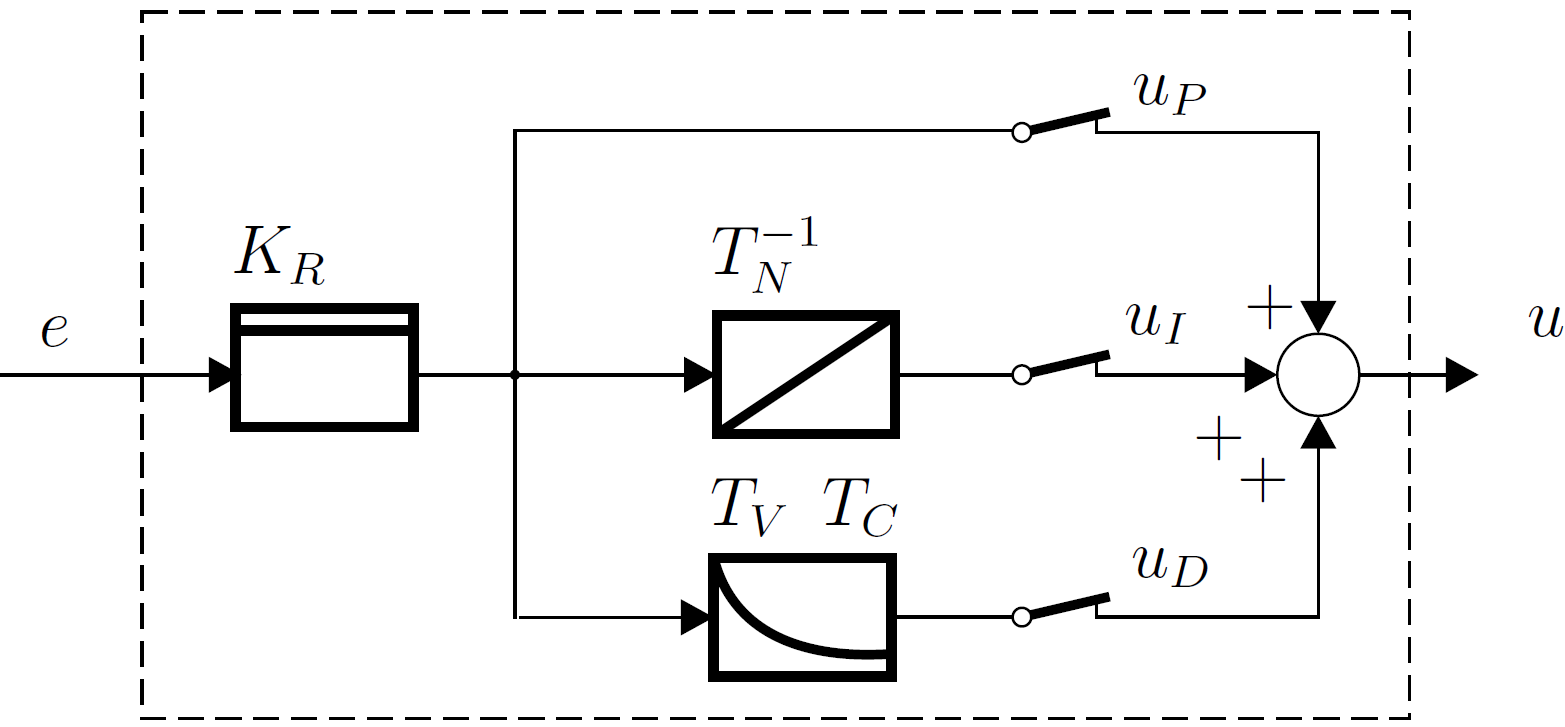
\includegraphics[width=\columnwidth]{images/pid_regler_aufbau_standardform.png}
\end{minipage}
\hfill
\begin{minipage}[c]{0.55\columnwidth}
    $$ \boxed{ G_{\rm PID}(\jimg \omega) = K_R + \Big( 1 + \frac{1}{\jimg \omega T_N} +\frac{\jimg \omega T_V}{1 + \jimg \omega T_C} \Big) } $$
\end{minipage}


\subsubsection{Variante 3: Serielle (multiplikative) Form}
\label{PID-Regler multiplikativ}

    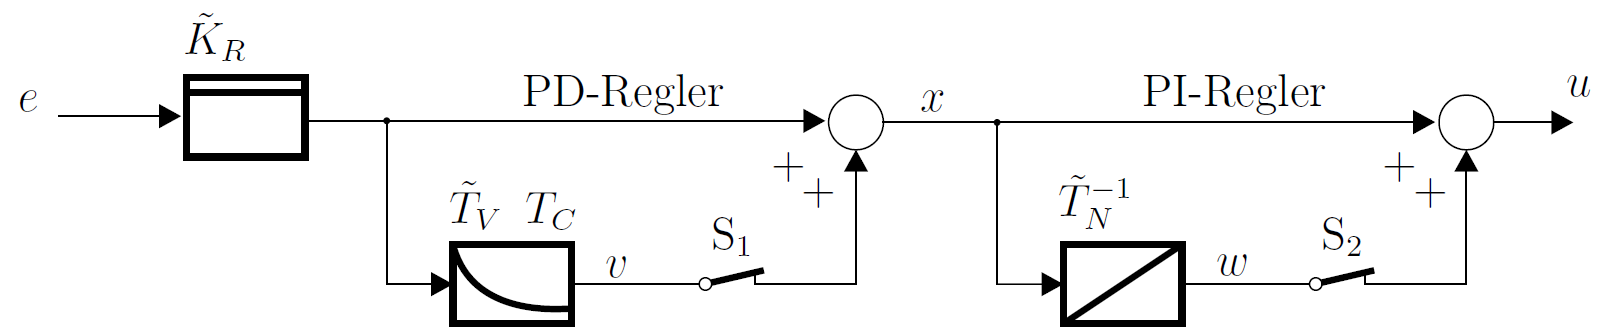
\includegraphics[width=0.8\columnwidth]{images/pid_regler_aufbau_serielle_form.png}
    $$ \boxed{ G_{\rm PID}(\jimg \omega) = \tilde{K}_R \cdot \Big( 1 + \frac{1}{\jimg \omega \tilde{T}_N} \Big) \cdot \Big(1 + \frac{\jimg \omega \tilde{T}_V}{1 + \jimg \omega T_C} \Big) } $$

\subsubsection{Umrechnung Parameter Variante 1 -- Variante 2}

\begin{tabular}{c c c c c c c c c}
    $K_R = K_P$ & & $T_N = \frac{K_P}{K_I}$ & & $T_V = \frac{K_D}{K_P}$ & & $K_I = \frac{K_R}{T_N}$ & & $ K_D = K_R T_V$
\end{tabular}

\subsubsection{Umrechnung Parameter Variante 2 -- Variante 3}

\begin{tabular}{c c c c c}
    $K_R = \tilde{K}_R \Big( 1 + \frac{\tilde{T}_V}{\tilde{T}_N} \Big)$ & &
    $T_N = \tilde{T}_N + \tilde{T}_V$ & &
    $T_V = \tilde{T}_V \frac{\tilde{T}_N - \tilde{T}_C}{\tilde{T}_N + \tilde{T}_V}$ 
\end{tabular}

\subsection{Matlab / Simulink}

\begin{minipage}[t]{0.45\columnwidth}
    \subsubsection*{Matlab}

    \begin{outline}
        \1 Parallelform
            \2 \mylstbox{C = pid(Kp, Ki, Kd, Tf)}
            \2 $C = K_p + \frac{K_i}{s} + \frac{K_d \cdot s}{T_f \cdot s + 1}$
        \1 Standardform
            \2 \mylstbox{C = pidstd(Kp, Ti, Td, N)}
            \2 $C = K_p \Big( 1 + \frac{1}{T_i \cdot s} + \frac{T_d \cdot s}{\frac{T_d}{N} s + 1} \Big)$
            \2 $T_f = \frac{T_d}{N}$
    \end{outline}
\end{minipage}
\hfill
\begin{minipage}[t]{0.53\columnwidth}
    \subsubsection*{Simulink}

    \begin{outline}
        \1 Parallelform
        \2 $P + I \frac{1}{s} + D \frac{N}{1 + N \frac{1}{s}}$
        \2 $D \frac{N}{1 + N \frac{1}{s}} = \frac{D \cdot s}{\frac{1}{N} s + 1}$
        \2 $P = K_P$, $I = K_I$, $D = K_D$, $N = \frac{1}{T_C}$
    \1 Standardform ('ideal')
        \2 $P \cdot \Big( 1 + I \frac{1}{s} + D \frac{N}{1 + N \frac{1}{s}} \Big)$
        \2 $D \frac{N}{1 + N \frac{1}{s}} = \frac{D \cdot s}{\frac{1}{N} s + 1}$
        \2 $P = K_R$, $I = \frac{1}{T_N}$, $D = T_V$, $N = \frac{1}{T_C}$
    \end{outline}
\end{minipage}


\subsection{PID-Regler im Frequenzgang}

\begin{outline}
    \1 \textbf{P}: Proportional $K_P$
        \2 Frequenz\textbf{un}abhängige Gewichtung
        \2 Allpassverhalten (alle Frequenzen gleich verstärkt)
    \1 \textbf{I}: Integral $K_I \frac{1}{\jimg \omega}$
        \2 Gewichtet tiefe Frequenzen stärker als hohe Frequenzen
        \2 Reagiert auf 'langsame' Änderungen 
        \2 Tiefpassverhalten; Phasenschiebung: $-90 \degree$ (im Uhrzeigersinn)
    \1 \textbf{D}: Differential $K_D \jimg \omega$
        \2 Gewichtet hohe Frequenzen stärker als tiefe Frequenzen
        \2 Reagiert auf 'schnelle' Änderungen 
        \2 Hochpassverhalten; Phasenschiebung: $+90 \degree$ (gegen Uhrzeigersinn)
\end{outline}


\subsection{PID-Regler im Bodediagramm}

\textbf{Achtung:} Gemäss den Frequenzgängen der verschiedenen Darstellungsformen aus Abschnitt ~\ref{Strukturen PID-Regler} 
eines PID-Reglers darf im Bodediagramm \textbf{nur Variante 3 grafisch aus den Einzelteilen addiert} werden. 
